\section{The Physics of Pre-Merger Evolution}

To preface Chapter \ref{ch:ch2}, which focuses on the merger remnants, we briefly cover a few topics related to evolution of the CO WD binary leading up to and during the early phases of the merger that are only considered in passing in subsequent chapters.  These include estimates on the typical WD masses involved in a typical CO WD binary merger, and the stability of mass transfer in interacting CO WDs.

\subsection{The CO WD Mass Range}
\label{ssec:cowd_massrange}

While we can roughly estimate the range of masses a CO WD can take as being between $\sim0.4$ and $\sim1.0\,\Msun$ (Sec. \ref{}), what are the typical masses involved in a CO WD merger?

%Statistically, mergers of certain types of WD binaries from Fig. \ref{wdbinarymasses} will dominate over others.  According to \cite{tremblay}, the mass distribution of DA white dwarfs (which comprise the vast majority of WDs) is narrowly peaked around $M = 0.65$ \Msun.  This suggests that the majority of WD binary interactions will be between near equal-mass CO WD pairs.  Binary evolution, however, will skew the population statistics of binary constituents.  \footnote{For example, in almost all cases a main-sequence binary system will undergo two stages of mass transfer to create a double degenerate system (one for the giant phase of each star).  The first phase of mass transfer must not result in common-envelope evolution; this requires a near-unity mass ratio between the two MS stars (see \cite{vkercj10} for details).  The most likely merger, then, is between two WDs of similar mass.}  \cite{han98} uses Monte Carlo simulations of binary evolution to determine that the birth rate of close-in WD binaries in the Milky Way is $\sim 3 \times 10^{-2}$ yr$^{-1}$, with 63\% being He-CO WD binaries, $\sim$ 2\% He-He, and 35\% CO-CO.  \citeauthor{han98} also gives merger rates: $5.7 \times 10^{-3}$ yr$^{-1}$ for He-He, $1.81 \times 10^{-2}$ yr$^{-1}$ for He-CO and $5.7 \times 10^{-3}$ yr$^{-1}$ for CO-CO mergers.  \cite{nele+01a}'s population sythesis models give different values for birth rates: a total rate of $4.8 \times 10^{-2}$ yr$^{-1}$, with 53\% of the binaries containing two He WDs, 25\% containing two CO WDs (including hybrid CO WDs with thick He envelopes), 20\% containing a CO and an He WD, and $\sim 1$\% containing ONeMg WDs.  The total merger rate for WDs of all sorts is $2.2 \times 10^{-2}$ yr$^{-1}$.  The differences between the two studies can be attributed to different common envelope inspiral efficiencies and treatments of mass transfer and stellar evolution.  (Each author also had multiple models with different treatments of such factors as star formation, WD cooling, etc.)

%http://adsabs.harvard.edu/abs/2015ApJ...815...63A
%https://arxiv.org/abs/1606.05292


\subsection{Merger Initial Conditions and Unstable Mass Transfer}
\label{ssec:stable_mass_transfer}

For all of the merger simulations we conduct in this thesis, we generate initial conditions by placing two unperturbed spherical WDs, whose rotation are unsynchronized with their orbital period, at an initial separation where the less massive WD's radius is equal to its Roche lobe (the radius around a star within which any material is gravitational bound to the star).  Note that the less massive WD is always the first to initiate mass transfer, since by the WD mass-radius relation,

\eqbegin
R \propto M^{\frac{1 - n}{3 - n}} \approx M^{-1/3}
\label{eq:c1_massradiusrelation}
\eqend

\noindent (approximating the low-mass cold WD EOS with an $n = 3/2$ polytrope), it is larger and therefore overflows its Roche lobe first.  The use of unsynchronized WDs was a choice first made in \cite{zhu+13} (Ch. \ref{ch:ch2}) in order to better compare with other simulations (specifically those of \citealt{loreig09}), and subsquently made in Ch. \ref{ch:ch3} and \ref{ch:ch4} to compare with Ch. \ref{ch:ch2}).  The consequences of this choice are discussed further in Sec. \ref{ssec:c2_initcond} and \ref{sec:c2_variation}.  

The use of spherical WDs, however, neglects the tidal bulges they develop close to the start of mass transfer.  As a result, once placed in the binary, the WDs deform and radially pulsate in response to the new potential, resulting in an overestimate of the rate of early mass transfer as material from the less massive WD overshoots the Roche lobe during each pulsation.  \cite{dan+11} show that ``accurate initial conditions'' that include tidal bulges extends the period of mass transfer prior to the full tidal disruption of the donor by several tens of orbital periods.  It much more difficult to accurately create tidal bulges in unsynchronized systems, and we discuss the effects of our ``approximate'' initial conditions in Sec. \ref{ssec:c2_importance_accurate_ics}.  The primary effect of using these is to misestimate the rate and duration of early mass transfer \citep{dsou+06, dan+11}, and its effect on the final inspiral phase and structure of the merger remnant will vary between mergers.\footnote{For example, \citeauthor{dan+11} (\citeyear{dan+11}, their Fig. 9) find the central density and temperature of the remnant from a $0.6-0.9\,\Msun$ merger changes by $\sim5$ and $\sim30$\%, respectively, when switching from approximate to accurate initial conditions, but \citeauthor{pakm+12sph} (\citeyear{pakm+12sph}, their Figs. 5 and 6) show few changes in the density and temperature profile during the final merger of a $1.0 - 1.1\,\Msun$ binary.}

% THESIS: We add here, however, that \cite{pakm+12sph} examined the differences between a synchronized WD binary mergers using accurate and approximate initial conditions.  They replicate \cite{dan+11}'s result that accurate initial conditions lead to mass transfer over dozens of orbits before the merger proper, the overall density structure of the system as well as the temperatures at the shear interface between the interacting WDs is nearly identical (\citealt{pakm+12sph}, Figs. 5 and 6).  Though dan+11 notes

Because mass transfer rates are overestimated, however, our simulations cannot predict which binaries will experience runaway mass transfer and merge -- indeed, every one of our simulations in Ch. \ref{ch:ch2} does so.  Whether or not mass transfer between two stars is stable has long been studied analytically and semi-analytically, and it is known that transfer depends critically on the mass ratio $\qm = \Md/\Md$ between the donor star (\Md) and the accretor star (\Ma; from above, $\Ma \geq \Md$ and $\qm \leq 1$ for all mergers), and whether or not spin and orbital angular momentum can be efficiently coupled to each other.  We sketch a simple argument for stability below.

Let us consider the case in which some dissipative process, such as tidal torquing between the donor and accretor or an accretion disk, is able to return any angular momentum from the WD spin back to orbital angular momentum, thus helping to stabilize mass transfer.  This means that $\dot{J}_\mrm{orb} = 0$.  The orbital angular momentum of a binary system is $J_\mrm{orb} = (\Ma\Md/\Mtot)\sqrt{G\Mtot a}$, where $\Mtot = \Md + \Ma$ and $a$ is the orbital separation.  From this we may derive $\dot{J}_\mrm{orb}/J_\mrm{orb} = \dot{\Md}/\Md + \dot{\Ma}/\Ma - \dot{M}_\mrm{tot}/2\Mtot + \dot{a}/2a$.  We shall assume conservative mass transfer (this is backed by the simulations in Ch. \ref{ch:ch2} and \ref{ch:ch3}, which show less than $1$\% of stellar material becomes unbound), meaning $\dot{\Ma} = -\dot{\Md}$.  Putting this together gives us

\eqbegin
\dot{J}_\mrm{orb}/J_\mrm{orb} = 2(\qm- 1)\frac{\dot{\Md}}{\Md} - \frac{\dot{a}}{a},
\label{eq:c1_adotovera}
\eqend

\noindent noting that $\dot{J}_\mrm{orb}/J_\mrm{orb} = 0$.  We use \cite{pacz71}'s estimate for the Roche lobe of \Md, $R_L \approx 0.46a(\Md/\Mtot)^{1/3}$, valid for $\qm \lesssim 1$ \citep{eggl83}.  Differentiating and using Eqn. \ref{eq:c1_adotovera}, we obtain

\eqbegin
\frac{\dot{R}_\mrm{L}}{R_\mrm{L}} = 2(\qm- \frac{5}{6})\frac{\dot{\Md}}{\Md}.
\label{eq:c1_rochedotoverroche}
\eqend

\noindent For mass transfer to be stable, \Rd\ must expand more slowly than $R_L$, or $\dot{R}_\mrm{d}/\Rd < \dot{R}_\mrm{L}/R_\mrm{L}$.  From Eqn. \ref{eq:c1_massradiusrelation}, $\dot{R}_\mrm{d}/\Rd = -\dot{\Md}/3\Md$; combining this with Eqn. \ref{eq:c1_rochedotoverroche}, we obtain the stability criterion $2(\qm- 5/6) < -1/3$, or:

\eqbegin
\qm < \frac{2}{3}.
\label{eq:c1_qcrit}
\eqend

\noindent Most of the systems we simulate, in particular the ones between WDs of mass $\sim0.65\,\Msun$, fall well outside of the stable regime, but a number (such as the $0.4 - 1.0\,\Msun$ merger in Ch. \ref{ch:ch2}) do satisfy this, and naively should not merge.

In the case where spin and orbital angular momentum coupling is instead negligible -- which implies that the accretion stream does not form a disk but rather directly impacts the accretor \citep{nele+01} -- a similar analysis can be peformed, using total angular momentum $J = J_\mrm{orb} + J_{spin} = (\Ma\Md/M)\sqrt{GMa} + J_{spin}$, from which we may derive $\dot{J}/J_\mrm{orb} = \dot{\Ma}/\Ma + \dot{\Md}/\Md - \dot{M}/2M + \dot{a}/2a + \dot{J}_{spin}/J_\mrm{orb}$.  Following \cite{marsns04} and \cite{nele+01}, we assume only the spin of the accretor matters for the equation, and follow \cite{verbr88}'s representation of the spin-up of the accretor from direct impact accretion with $\dot{J}_{spin} = -\sqrt{G\Ma R_h}\dot{\Md}$ ($\dot{\Md}$ is negative).  $R_h$ is the effective radius of the matter transferred onto the accretor, and the ratio $r_h = R_h/a$ is given by a fitting formula: $r_h = 0.0883 - 0.04858\log({q}) + 0.11489{\log}^2(q) + 0.020475{\log}^3(q)$, valid for all plausible WD binary mass ratios \citep{verbr88}.  Dividing this by $J_\mrm{orb}$ to obtain $\dot{J}_{spin}/J_\mrm{orb} = -\sqrt{(1 + q)r_h}\dot{\Md}/\Md$, and assuming conservative mass transfer ($\dot{J} = 0$), we obtain \citep{marsns04,nele+01}

\eqbegin
\frac{\dot{a}}{a} = 2\left(\qm- 1 + \sqrt{(1 + q)r_h}\right)\frac{\dot{\Md}}{\Md}.
\label{eq:c1_adotovera2}
\eqend

\noindent Using the same argument that gave us Eqn. \ref{eq:c1_qcrit},

\eqbegin
2\left(\qm- \frac{5}{6} + \sqrt{(1 + q)r_h}\right) < - \frac{1}{3},
\label{eq:c1_qcrit2}
\eqend

\noindent which, solved numerically, is

\eqbegin
\qm\lesssim 0.219,
\label{eq:c1_qcrit3}
\eqend

\noindent well-below any mass ratio for a CO WD binary (from Sec. \ref{ssec:cowd_massrange}).  Eqns. \ref{eq:c1_qcrit} or \ref{eq:c1_qcrit3} represent the upper and lower-bounds of mass transfer stability, as seen in Fig. \ref{fig:c1_stability}: a binary with $\qm > 2/3$ will experience unstable mass transfer even with perfect angular momentum coupling, while a binary with $\qm \lesssim 0.2$ will always be stable, even with no coupling.  The critical $\qm$ for an imperfect coupling will fall somewhere between these two.

\begin{figure}
\centering
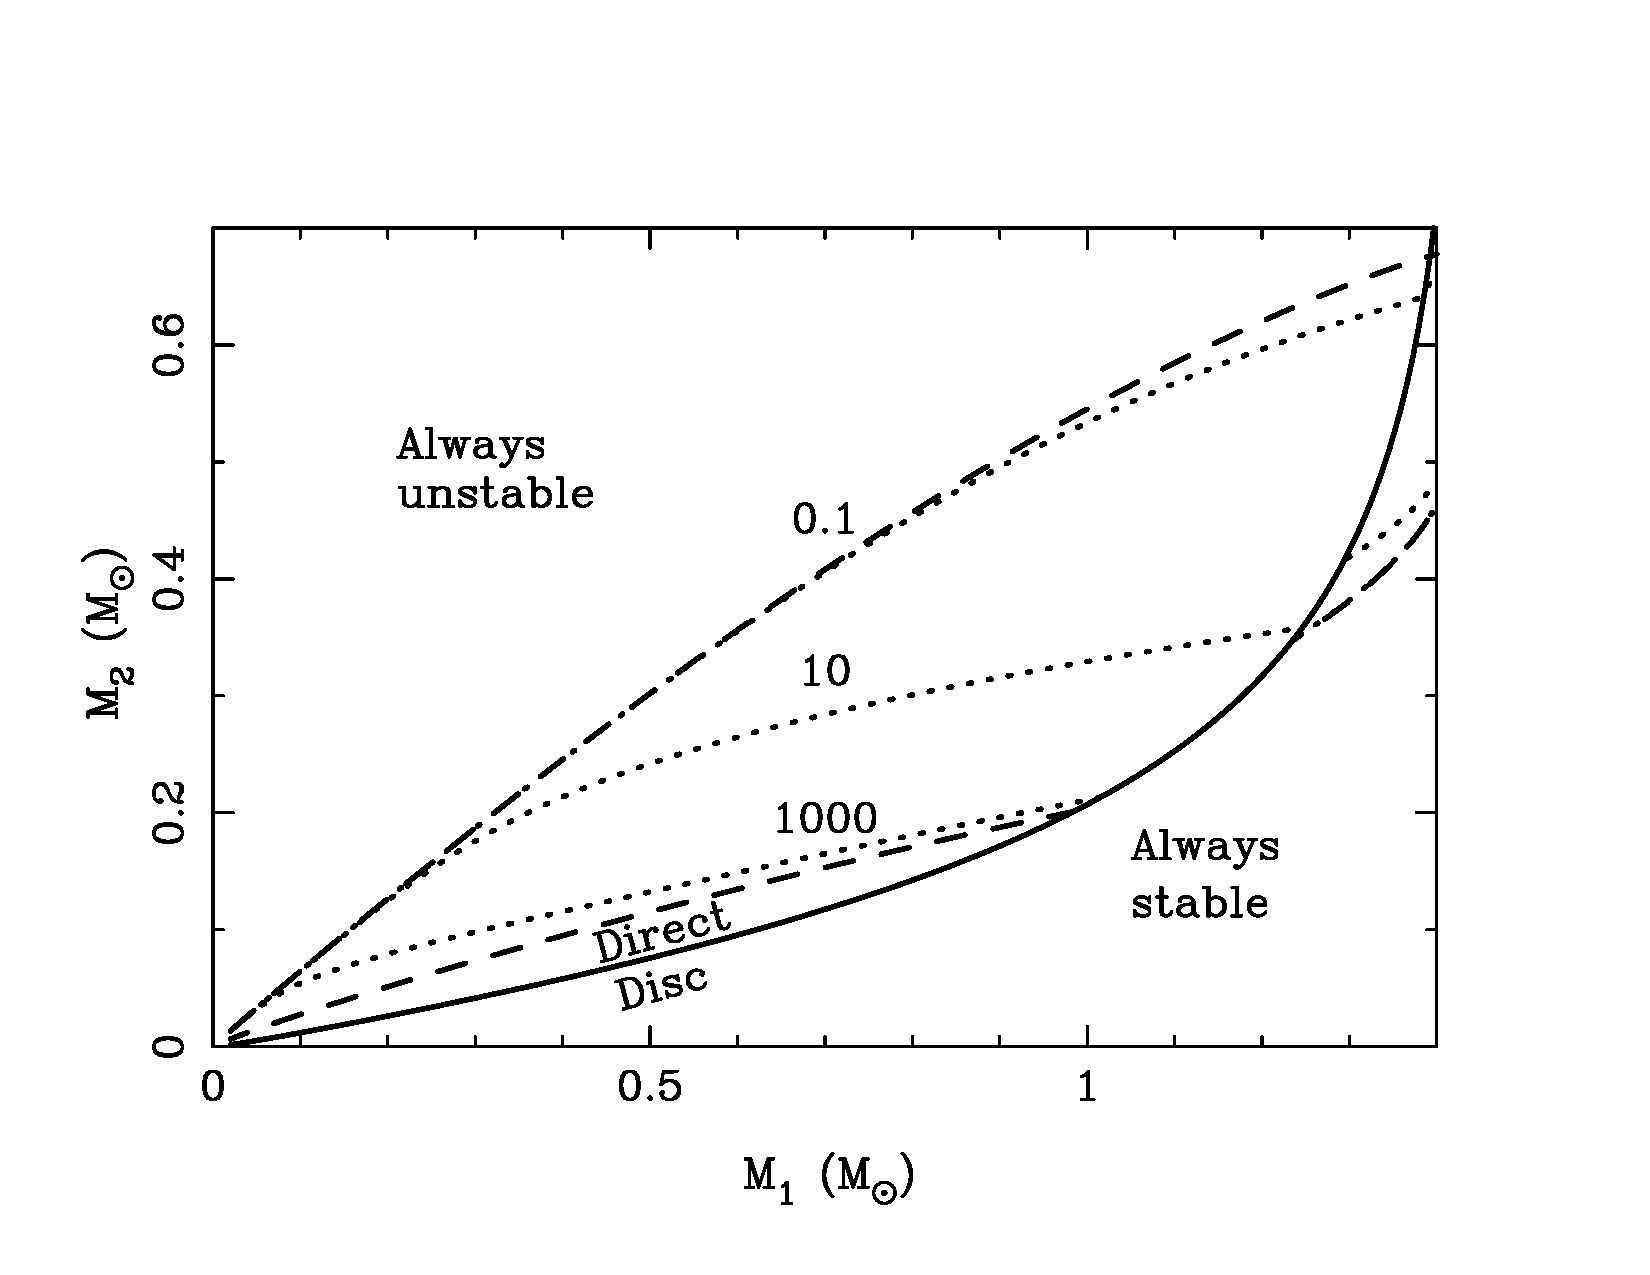
\includegraphics[angle=0,width=0.6\columnwidth]{introduction/figures/marsns04_stab.pdf}
\caption{Regions of stable and unstable mass transfer for the WD merger parameter space from \citeauthor{marsns04} (\citeyear{marsns04}; their Fig. 1).  $M_1$ is \Ma\, and $M_2$ is \Md.  The upper dashed line is a more accurate estimate for Eqn. \ref{eq:c1_qcrit}, and the lower dashed one that for Eqn. \ref{eq:c1_qcrit2}.  The solid line represents transition between direct impact and disk accretion.  Dotted lines represent the transition from stable to unstable mass transfer when the tidal synchronization timescale $\tau_\mrm{s}$ is $1000$, $10$ and $0.1\,\mrm{yr}$.}
\label{fig:c1_stability}
\end{figure}

The question then becomes which stability better represents mass transfer in WD binaries.  In the absence of other sources of spin-orbit coupling, this is determined solely by whether disk or direct impact accretion occurs.  Following \citep{lubos75}, \citep{nele+01} determines when one transitions into the other by calculating the point where the minimum radius reached by the accretion stream becomes larger than the accretor; the corresponding critical surface in the merger mass parameter space is plotted in Fig. \ref{fig:c1_stability}.  For $0.4 \leq \Ma \leq 1.0$, the line falls below $\qm = 0.1$, well below even Eqn. \ref{eq:c1_qcrit3}.

Tides within the WDs can substitute disks for spin-orbit coupling.  While traditional estimates of the spin-orbit synchronization timescale in WD binaries ranges from $\tau_{S} \sim 10^{12}$ yr for radiative damping to $\tau_{S} \sim 10^{15}$ yr for molecular viscosity \citep{marsns04}, other sources of dissipation, such as turbulent viscosity \citep{mochl89}, may lead to much shorter $\tau_{S}$.  Recent work \citep{fulll12, burk+13, fulll14} that resonant coupling between tidal forces and stellar pulsations favor a much shorter $\tau_\mrm{s}$ (though exactly how short remains unclear; \citealt{fulll14}).  Semi-analytical calculations \citep{marsns04,gokhpf07, kermsk15} suggest that even for $\tau_\mrm{s}$ as small as $10\,\mrm{yr}$, however, all the systems we consider in this thesis should still experience unstable mass transfer and merge.  All these systems also merge in simulations that more accurately model the binary at the onset of mass transfer \citep{dan+11, dan+12}, and so we proceed under the notion that all our binaries should merge.  We note that there is evidence \citep{shen15, brow+16} that even He - CO WD binaries with extremely low $\qm$ do so as well.

% THESIS NOTE: While recent merger simulations have favored synchronized initial conditions (rask+12, 14, dan+12, 14), whether or not tides can sychronize WD binaries remains an open question (dan+14, 2016ApJ...821...67S).  Moreover, dan+14 find that during the merger itself, neither WD is able to maintain its spin against its orbital period as the WD separation reduces dramatically over only a few binary orbits.

%Estimates of the synchronization timescale in binary systems give $\tau_{S} \sim 10^{12}$ yr from radiative damping, and $\tau_{S} \sim 10^{15}$ yr from viscosity \citep{marsns04}.  To compare, the timescale for angular momentum loss from gravitational wave radiation is \citep{segrcm97}

%\noindent In the latter stages of evolution, this value is around $\tau_{S} \sim 10^{6}$ yr.  It is then likely that neither donor nor accretor are synchronized at the time of merger\footnote{A close-in WD binary should merger within $10^8$ to $10^9$ yrs after formation \cite{segrcm97}.  Of course, any transients caused by mergers seen today must have occured within this time!}.  Turbulent viscosity and non-radial mode excitation, on the other hand, can potentially have $\tau_{S} << 500$ yr, and even small magnetic fields, properly oriented, can significantly enhance viscosity \citep{marsns04,ibentf98}.  Also, the viscous timescale scales as $a^6$, while Eqn. \ref{gravtimescale} scales as $a^4$; this indicates that should viscosity ever synchronize a WD binary, this binary will be synchronized for the remainder of its inspiral \citep{ibentf98}.  Whether or not a binary will be synchronized is still largely an unsolved problem \citep{mars11}.

%If we were to suppose a WD system could synchronize, then viscous dissipation should heat up both WDs significantly.  \cite{ibentf98} perform long equal-mass binary evolution calculations that assumes the binary system is synchronized, and the rate of tidal heating is equal to the rate of spin kinetic energy increase. (SO DOES IT SAP ROTATION????)  They find that over the course of the last $10^4$ yrs before merger heating from synchronization can increase the temperature of a 1.0 {\Msun} (with a 1.0 {\Msun} companion) by an order of magnitude.  While most of the thermal energy that is radiated away during this heat-up is in the form of neutrinos, the EM luminosity increases by almost five orders of magnitude.  At the time of merger, each 1.0 {\Msun} WD would shine with $\sim 100$ L$_{\odot}$ and have a temperature of $\sim 10^8$ K, making the system a significant X-ray source.  The luminosity just before merger increases with WD mass, and the period of time over which luminosity increase occurs drops with WD mass: a 0.3 {\Msun} with an equal-mass companion will increase in luminosity by two orders of magnitude over $10^6$ yr.  If the efficiency by which rotational energy is converted to thermal energy is reduced to 10\% the maximum efficiency in the 1.0-1.0 {\Msun} binary, the final luminosity drops by a factor of about 1000.  In all cases simulated, \citeauthor{ibentf98} found temperatures were insufficient to ignite nuclear fusion.  The periods of increased luminosity are all in the range of $10^2 - 10^6$ years, which, while short compared to the liftime of the binary, are far too long to be considered transients.


